\chapter{Experimental Validation}
\label{chapter:experiments}

\section{Setup}
\label{sec:setup}

To validate our implementation, we performed a series of experiments with various configurations and compared the results against classical simulations.
\begin{itemize}
    \item A 1D simulation with a constant velocity field
    \item A 2D simulation with a non-uniform velocity field
    \item A 3D simulation with a non-uniform velocity field
    \item A 2D simulation with non-uniform, time-varying velocity field and non-standard link velocities.
\end{itemize}
For details on the specific configurations that might be omitted, please refer to the code repository.
The full RMSE plots for all experiments are available in Appendix \ref{app:rmse}.

The method was implemented using Qiskit \cite{qiskit2024} and validated using the statevector simulator.
The QLBM simulator was implemented by us previously, adapting and extending the work of \cite{wawrzyniak2025base}.
All code is open source and available at \url{https://github.com/widdrr/qlbm}

\section{Simulations Without Boundary Conditions}
\label{sec:exp-no-bc}

\paragraph*{1D Simulation}
The QLBM configuration used was a standard 1DQ3 with 32 lattice sites.
The initial distribution is a simple Gaussian hill and the velocity field is a constant $u=0.3$.

\begin{figure}[H]
    \centering
    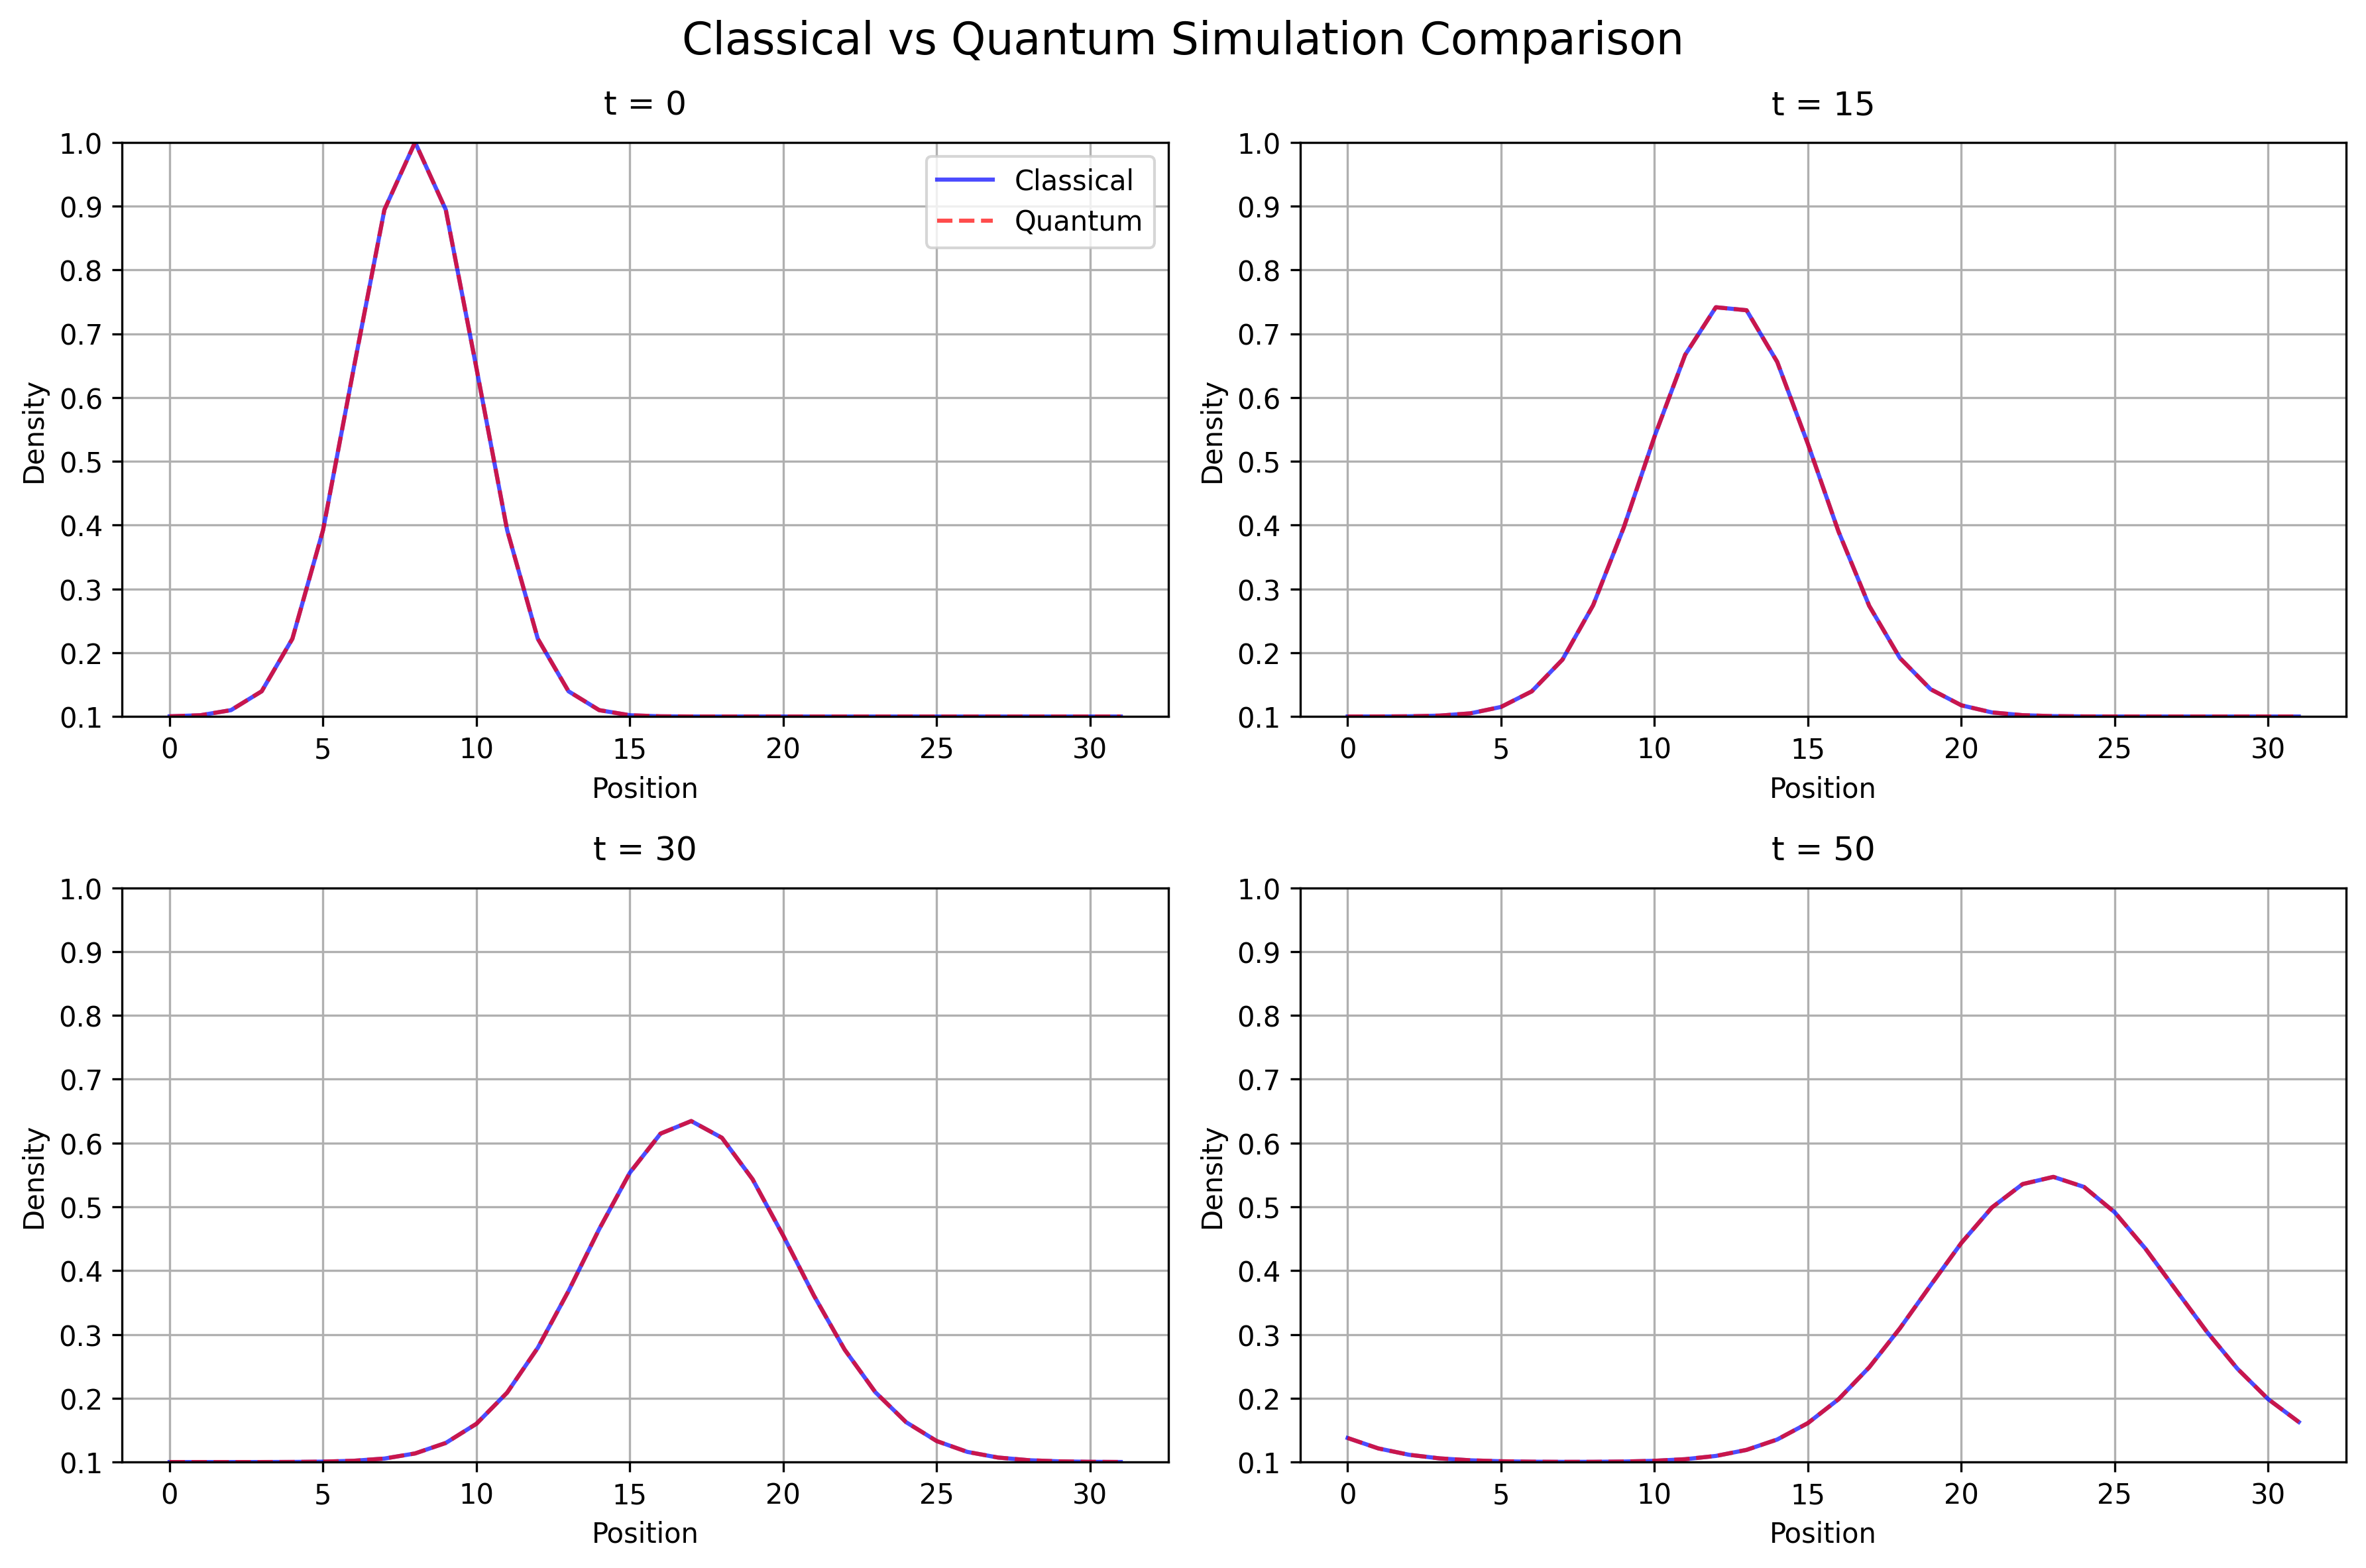
\includegraphics[width=\textwidth]{src/img/figures/1_Dcomparison.png}
    \caption{Comparison of quantum and classical simulations for the 1D case}
    \label{fig:1d_comparison}
\end{figure}

This experiment showed exact agreement between the quantum and classical simulations, with the RMSE in the order of $10^{-13}$ attributed to numerical errors.

\paragraph*{2D Simulation}
The QLBM configuration used was a standard 2DQ9 with $32 \times 16$ lattice sites.
The initial distribution is a ring of higher density and the velocity field consists of constant $u = 0.2$ in the bottom half and $u=-0.2$ in the top half with a constant $v=0.1$.

\begin{figure}[H]
    \centering
    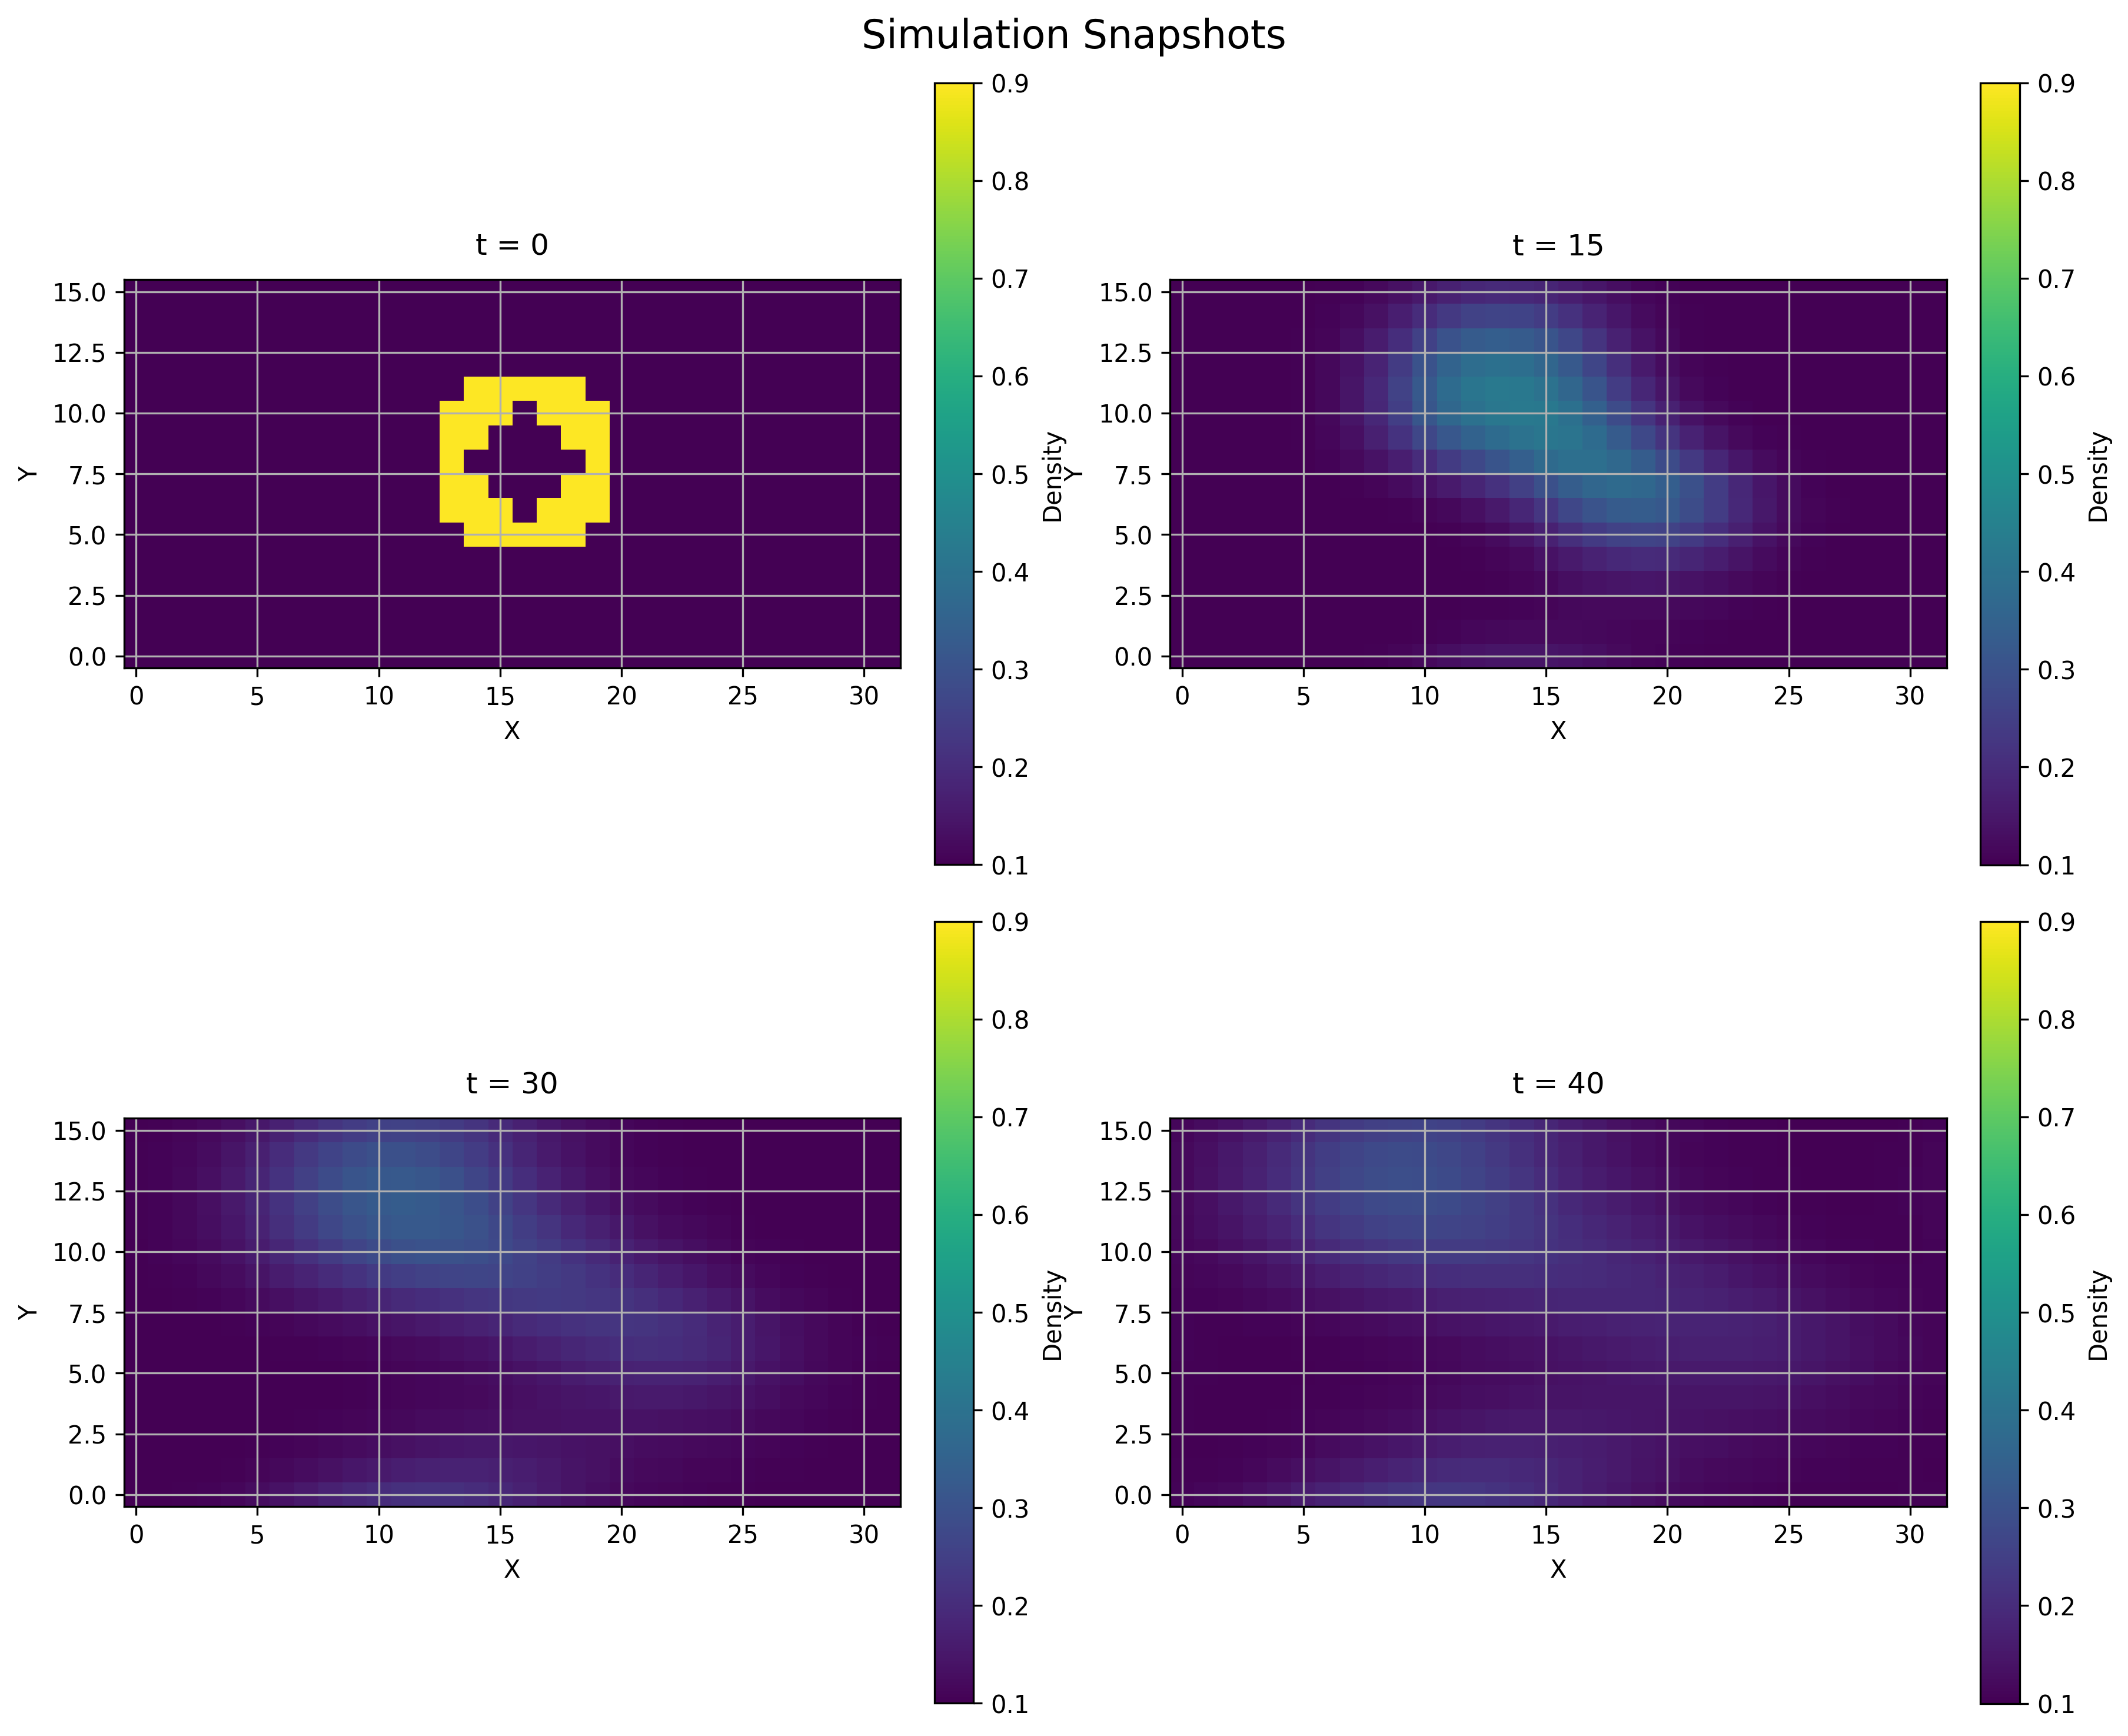
\includegraphics[width=\textwidth]{src/img/figures/2_Dquantum.png}
    \caption{Heatmap evolution of the 2D simulation with non-uniform velocity field}
    \label{fig:2d_snapshots}
\end{figure}

Once again, the numerical differences are negligible at $10^{-13}$.

\paragraph*{3D Simulation}
The QLBM configuration used was a standard 3DQ27 with $8 \times 8 \times 8$ lattice sites.
The initial distribution is three perpendicular planes of higher density and the velocity field follows the pattern:

\begin{align}
    u(x,y,z) &= A \cos(ax)\sin(by)\sin(cz) \\
    v(x,y,z) &= B \sin(ax)\cos(by)\sin(cz) \\
    w(x,y,z) &= C \sin(ax)\sin(by)\cos(cz)
\end{align}

With $A=B=C=0.2$ as the velocity amplitudes and $a=b=c=1.0$ as the spatial frequencies.

\begin{figure}[H]
    \centering
    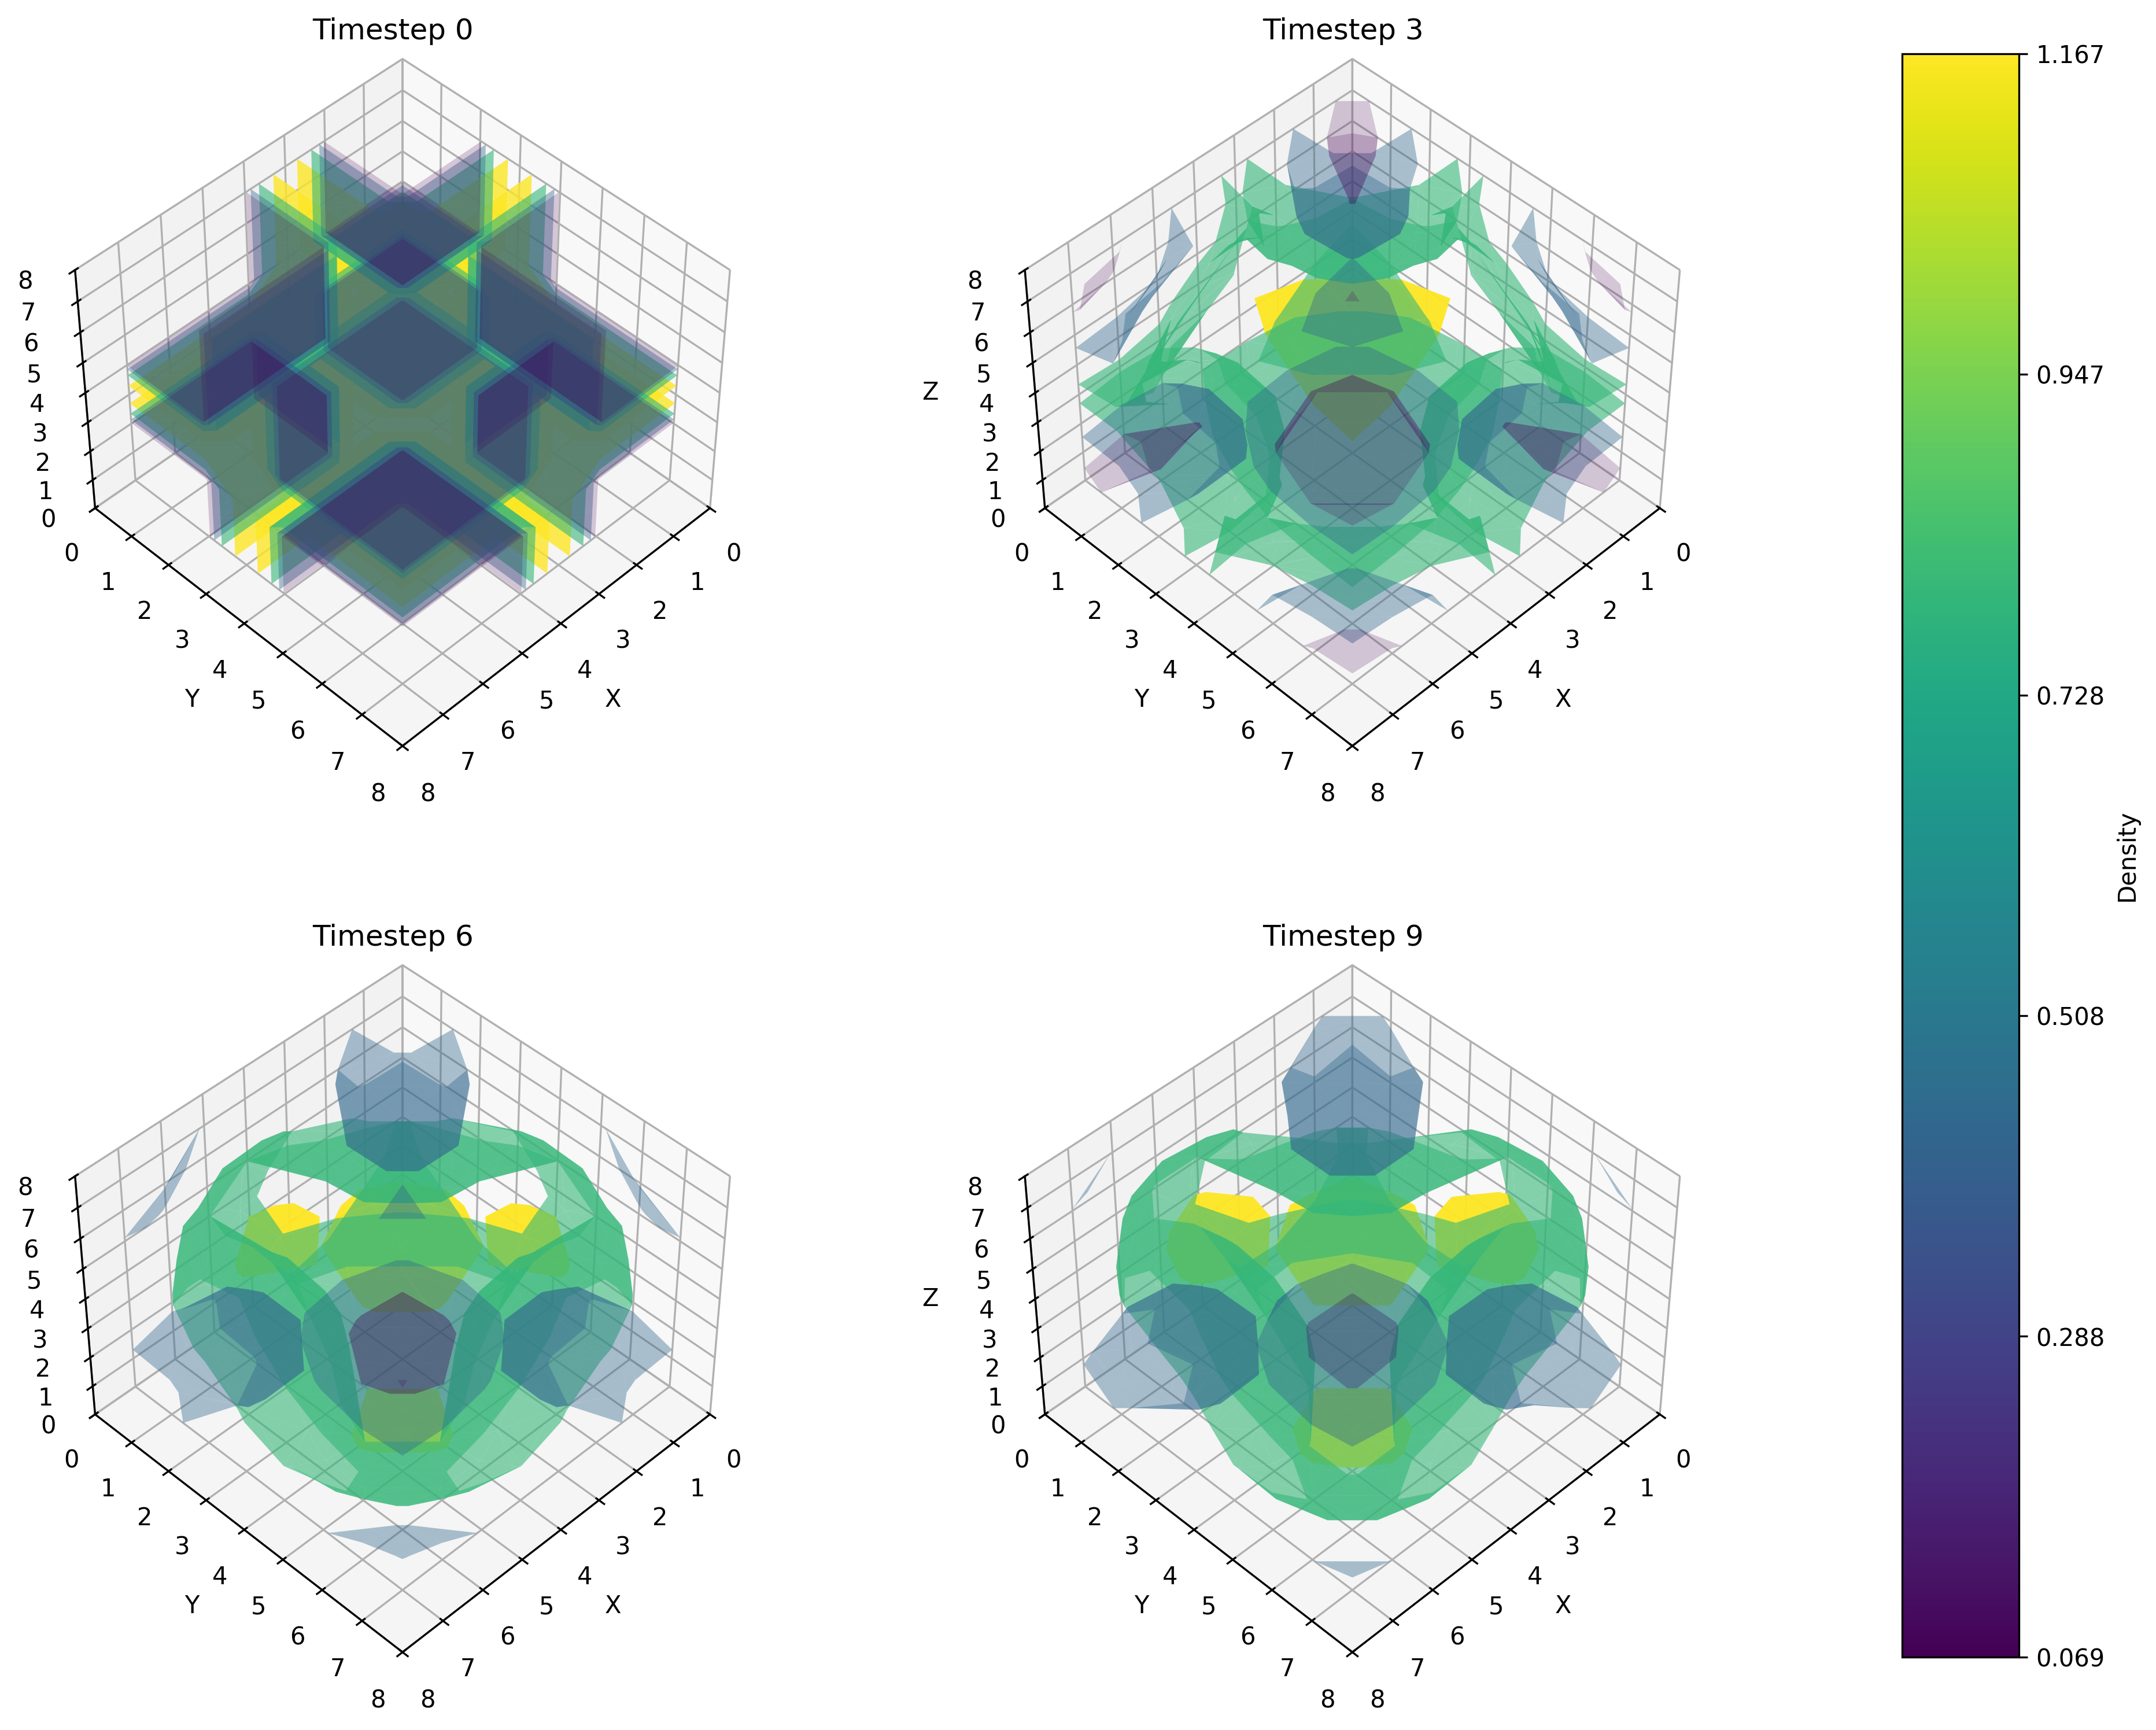
\includegraphics[width=\textwidth]{src/img/figures/3_Dquantum_snapshots.png}
    \caption{Isosurface evolution of the 3D simulation with non-uniform velocity field}
    \label{fig:3d_snapshots}
\end{figure}
The RMSE for this simulation is considerably higher at around $10^{-5}$, but still within acceptable limits.
This is attributed to the more complex velocity field.

\paragraph*{2D Simulation with Non-Standard Link Velocities}
The number of lattice sites is $32 \times 32$.
The initial distribution is a cross of higher density.

The configuration changes during the simulation in the following manner:
\begin{itemize}
    \item For the first 15 iterations, the standard 2DQ9 link velocities are used and the velocity field is a clockwise rotation vortex of magnitude $u=0.5$.
    \item For the next 10 iterations, the velocity field disappears and the link velocities are changed to the non-standard set $[(0,0), (2,1), (-2,-1)]$, restricting propagation to a single diagonal direction.
\end{itemize}

\begin{figure}[H]
    \centering
    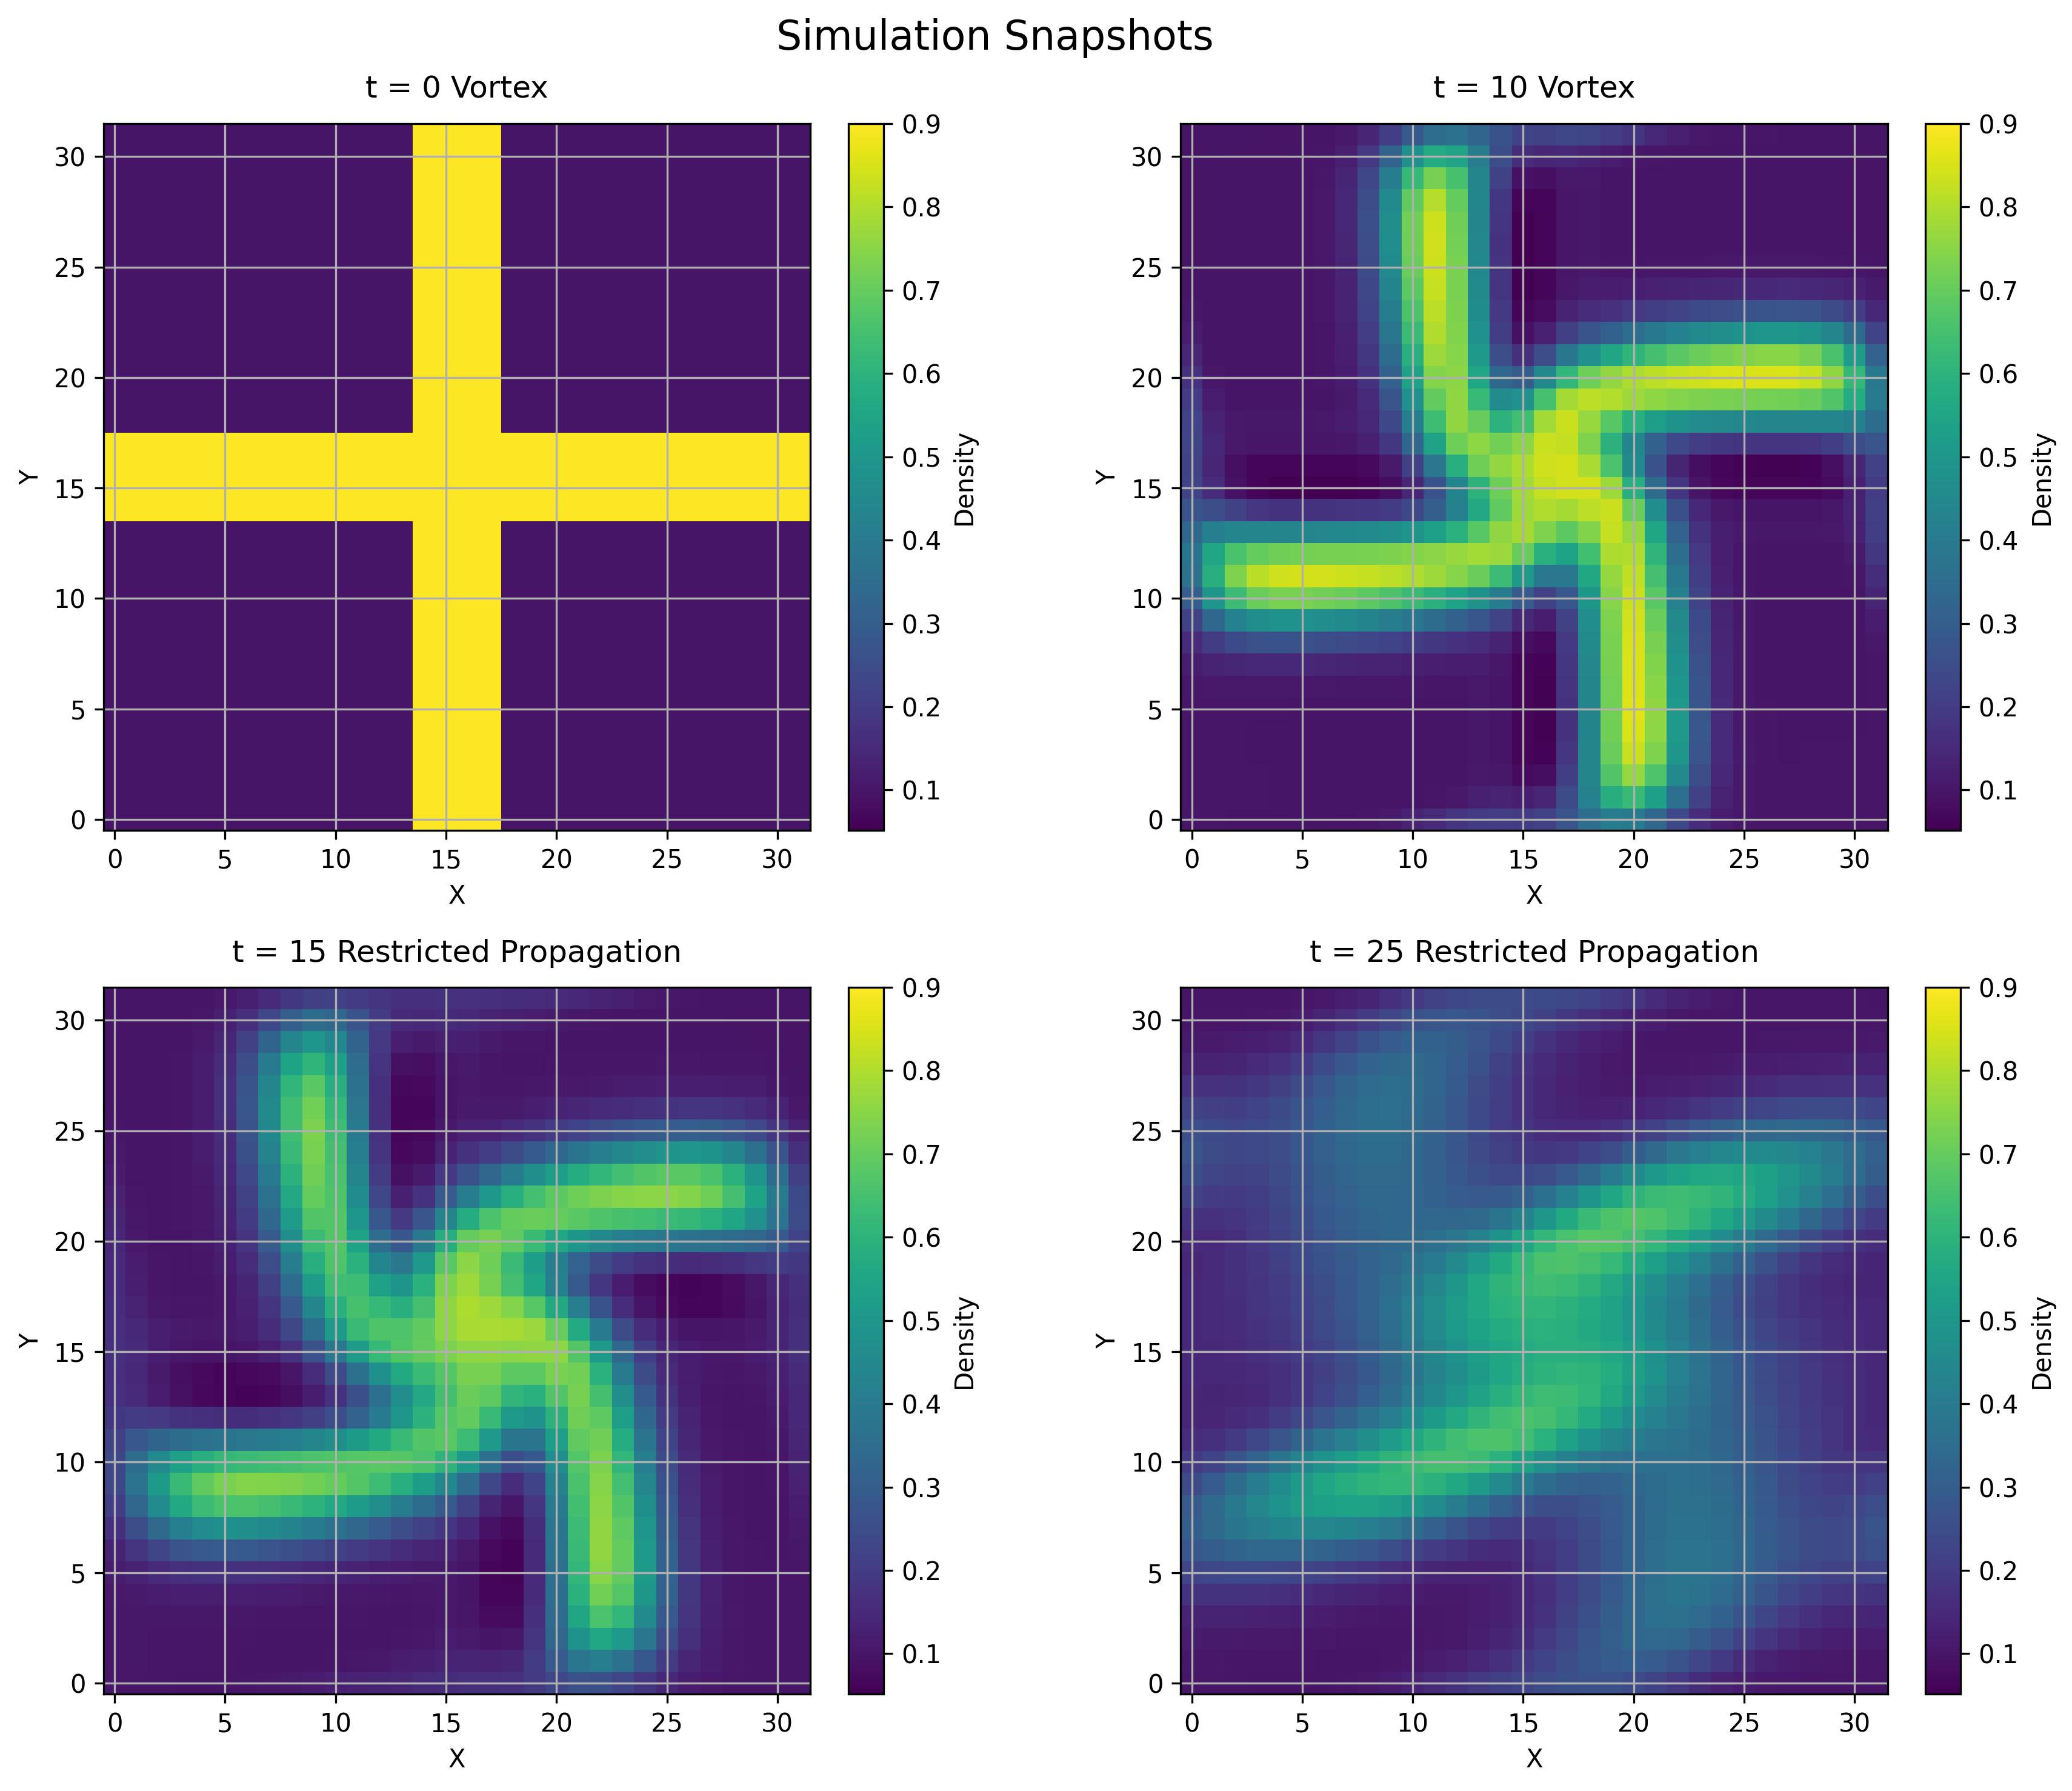
\includegraphics[width=\textwidth]{src/img/figures/cross_quantum_snapshots.png}
    \caption{Heatmap evolution of the 2D simulation with time-varying velocity field and non-standard link velocities}
    \label{fig:cross_snapshots}
\end{figure}

This simulation shows the highest RMSE of around $10^{-4}$. The more interesting part is that once the velocity field disappears at $t=15$, the error starts to decrease, as seen in Appendix \ref{app:rmse}.
This supports the hypothesis that the error is due to complex velocity fields.

\section{Simulations With Boundary Conditions}
\label{sec:exp-bc}

We validated the method using a 1D Advection-Diffusion setup.
This was chosen due to simplicity, but in theory nothing prevents the method from being applied to higher dimensions or more complex collision operators.
The simulation parameters were as follows:

\begin{itemize}
    \item \textbf{Lattice:} 1D grid, size 32.
    \item \textbf{Setup:} D1Q3 (Left, Rest, Right velocities).
    \item \textbf{Initial Condition:} Gaussian hill centered in the domain.
    \item \textbf{Velocity Field:} $u=0.1$ (rightward) for $t \in [0, 75]$, then $u=0$ for $t \in [75, 150]$.
    \item \textbf{Boundary Conditions:} Solid walls at both ends, populations that would stream into the boundary are instead redistributed to be stationary. Equations for right boundary:

    \[f_{-1}^{post} = f_{-1}^{pre} \]
    \[f_{0}^{post} = f_{0}^{pre} + 1.0 \cdot f_{1}^{pre}\]
    \[f_{1}^{post} = 0 \]
\end{itemize}

We performed both a classical simulation (implementing the same matrix logic) and the quantum simulation (statevector simulator).
The classical simulation visually matched the expected behavior of a solid wall.

\begin{figure}[H]
    \centering
    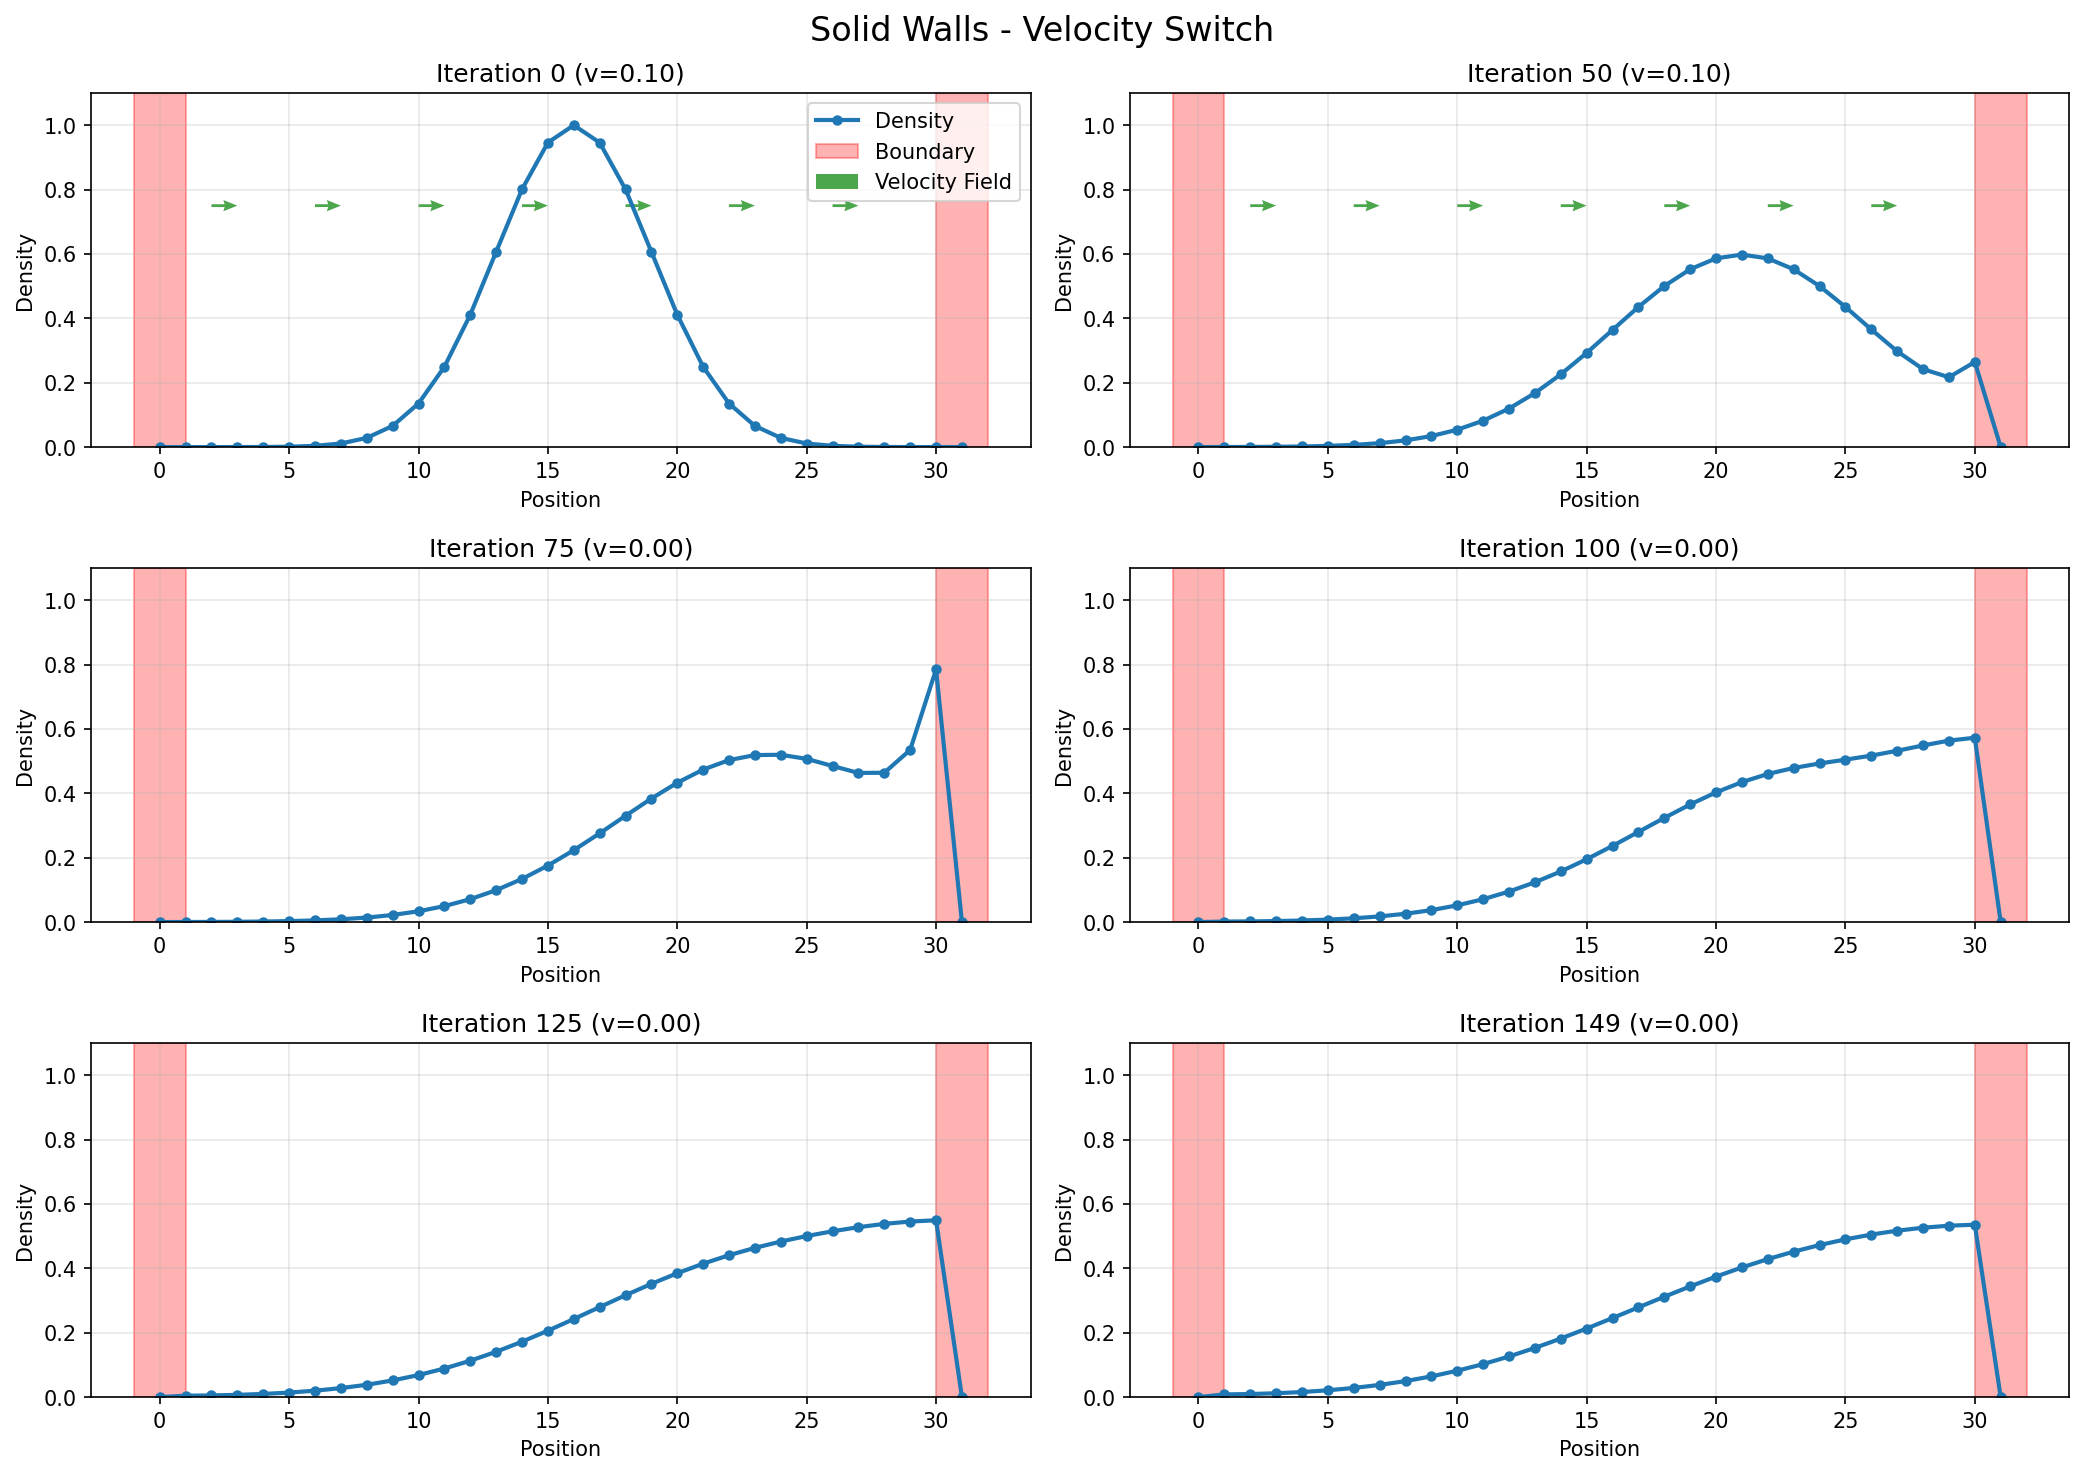
\includegraphics[width=0.8\textwidth]{src/img/figures/snapshots.png}
    \caption{Classical simulation results showing the Gaussian profile being contained by the solid walls. Given enough iterations, it would eventually flatten completely.}
    \label{fig:bc_snapshots}
\end{figure}

The quantum simulation was validated by computing the Root Mean Square Error (RMSE) between the classical and quantum results at each time step.

\begin{figure}[H]
    \centering
    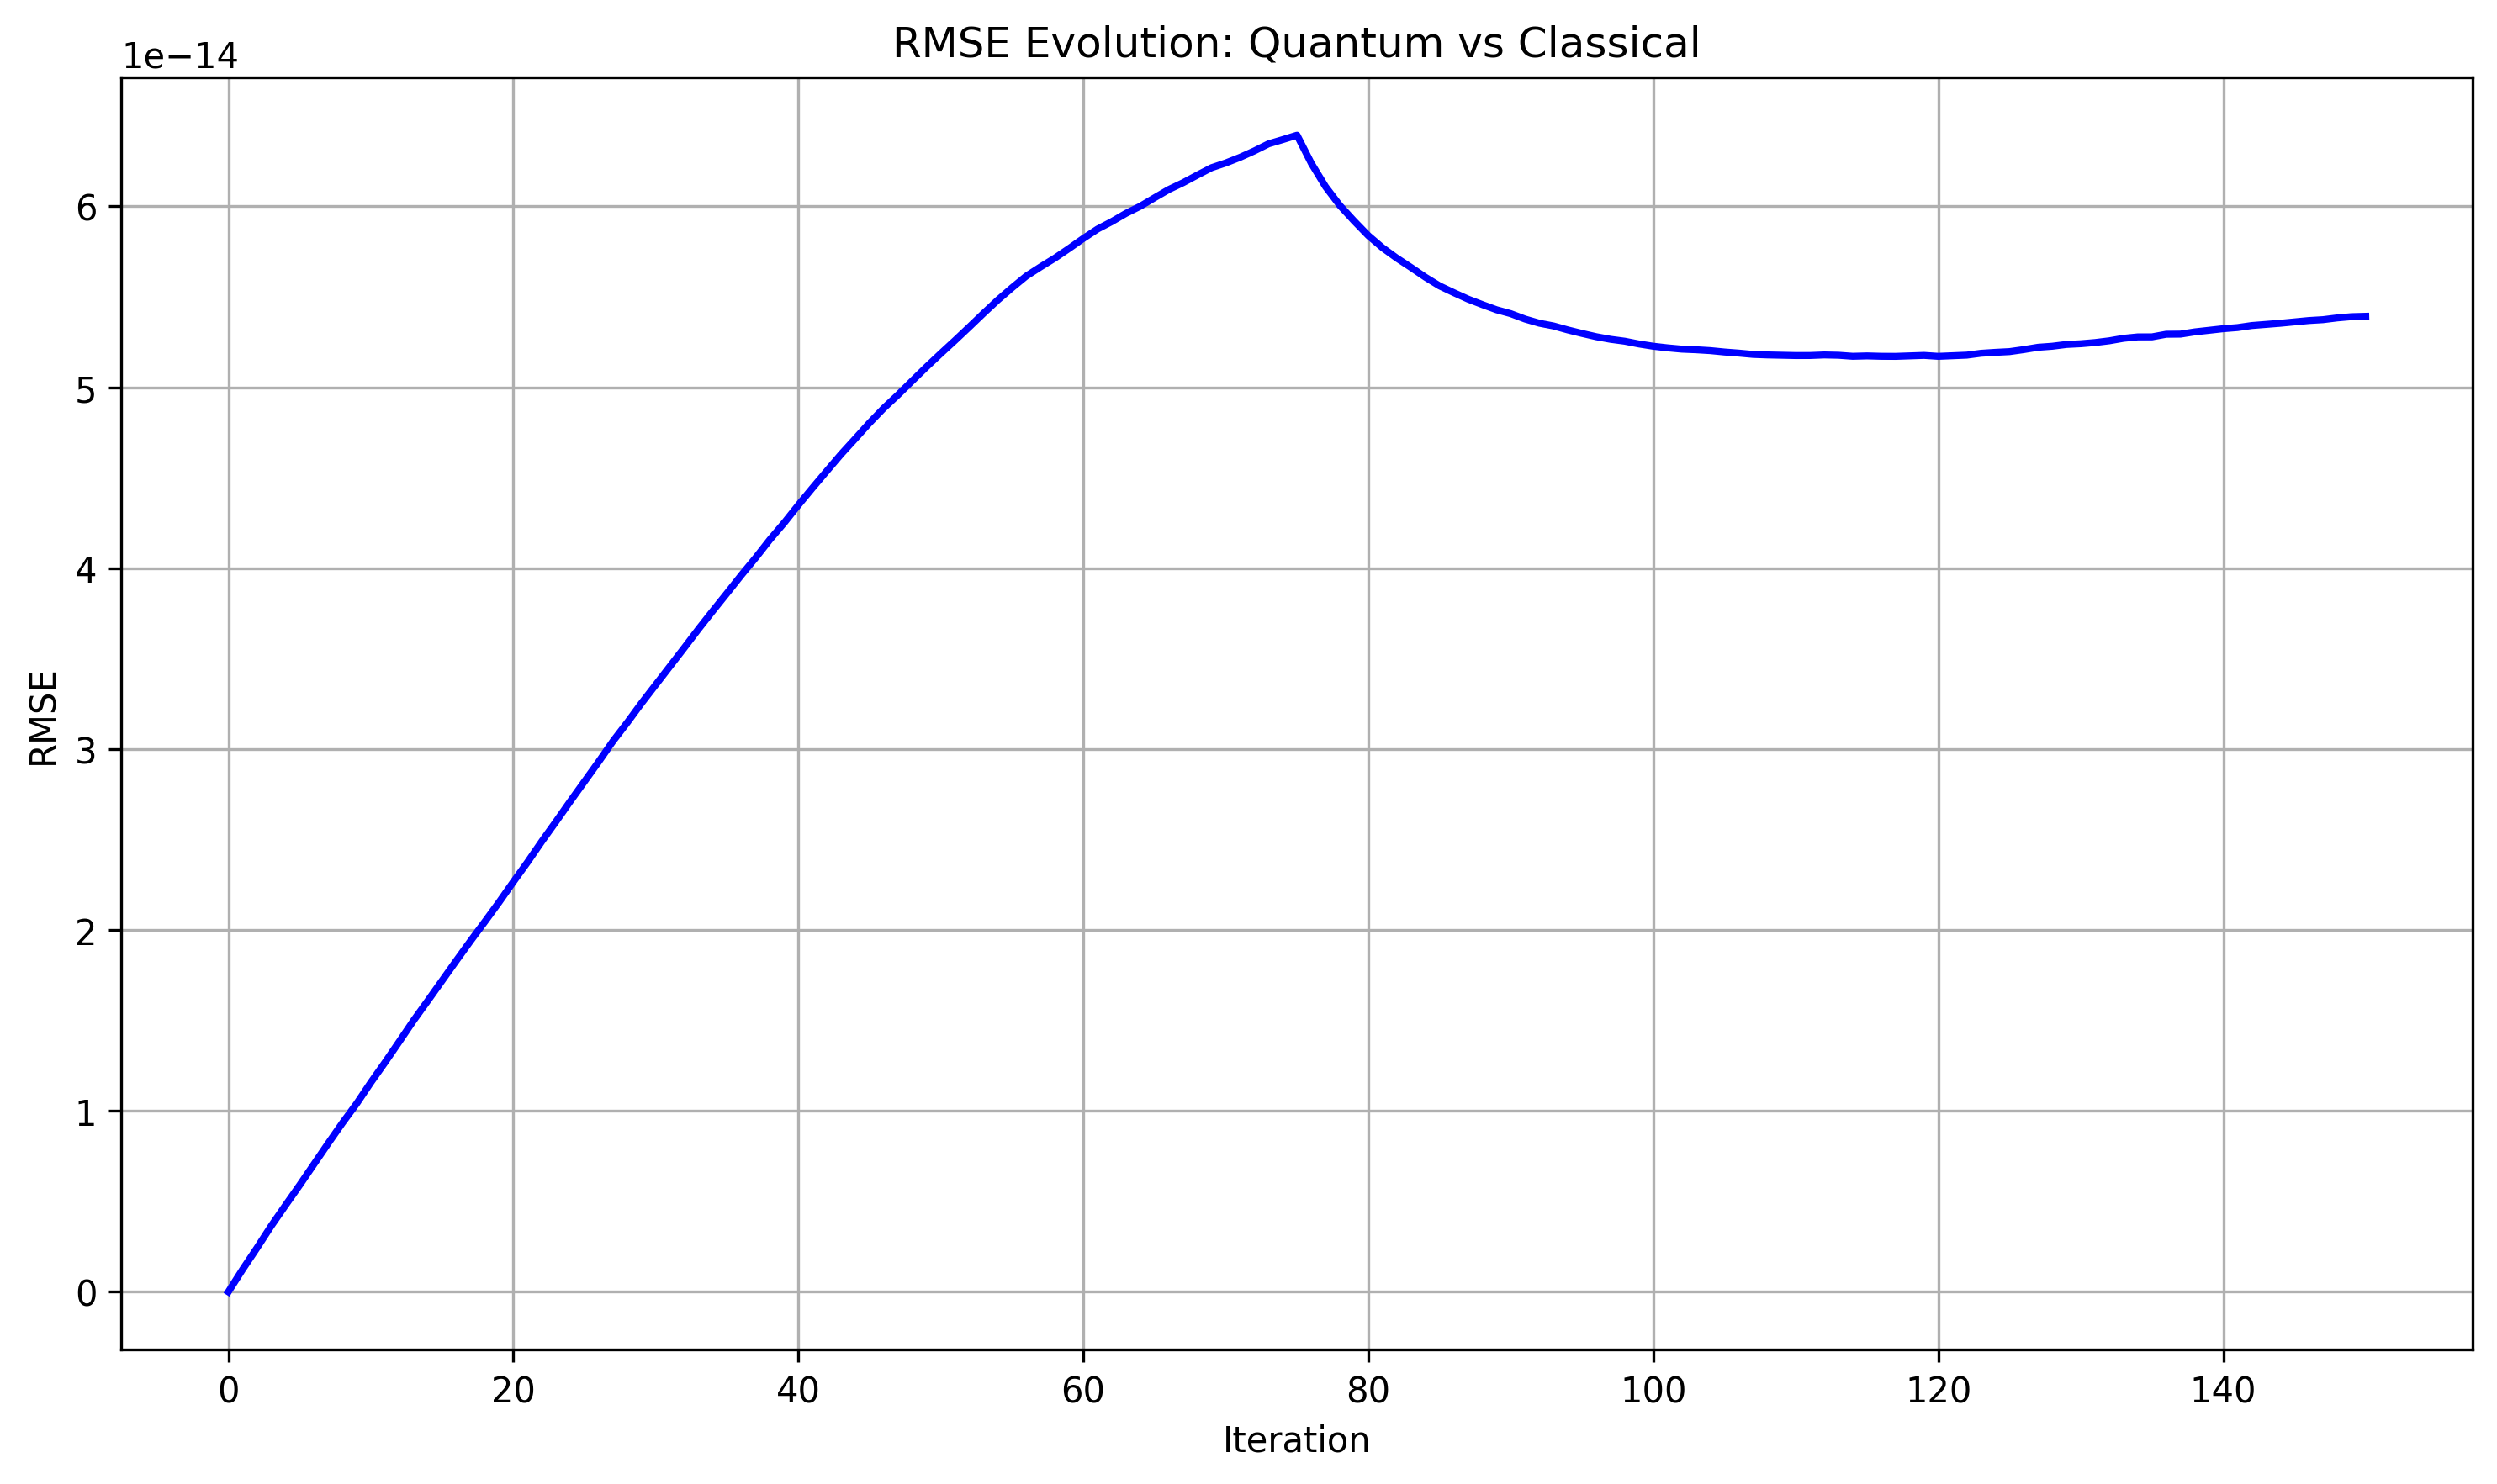
\includegraphics[width=0.8\textwidth]{src/img/figures/rmse_comparison.png}
    \caption{RMSE comparison between Classical and Quantum implementation demonstrating numerical precision agreement.}
    \label{fig:bc_rmse}
\end{figure}
